%%%%%%%%%%%%%%%%%%%%%%%%%%%%%%%%%%%%%%%%%
% Beamer Presentation
% LaTeX Template
% Version 1.0 (10/11/12) 
%
% This template has been downloaded from:
% http://www.LaTeXTemplates.com
%
% License:
% CC BY-NC-SA 3.0 (http://creativecommons.org/licenses/by-nc-sa/3.0/)
%
%%%%%%%%%%%%%%%%%%%%%%%%%%%%%%%%%%%%%%%%%

%----------------------------------------------------------------------------------------
%	PACKAGES AND THEMES
%----------------------------------------------------------------------------------------

\documentclass{beamer}

\mode<presentation> {
%\mode<handouts> {
%\mode<article> {


% The Beamer class comes with a number of default slide themes
% which change the colors and layouts of slides. Below this is a list
% of all the themes, uncomment each in turn to see what they look like.


%\usetheme{default}
%\usetheme{AnnArbor}
%\usetheme{Antibes}
%\usetheme{Bergen}
%\usetheme{Berkeley}
%\usetheme{Berlin}
%\usetheme{Boadilla}
\usetheme{CambridgeUS}
%\usetheme{Copenhagen}
%\usetheme{Darmstadt}
%\usetheme{Dresden}
%\usetheme{Frankfurt}
%\usetheme{Goettingen}
%\usetheme{Hannover}
%\usetheme{Ilmenau}
%\usetheme{JuanLesPins}
%\usetheme{Luebeck}
%\usetheme{Madrid}
%\usetheme{Malmoe}
%\usetheme{Marburg}
%\usetheme{Montpellier}
%\usetheme{PaloAlto}
%\usetheme{Pittsburgh}
%\usetheme{Rochester}
%\usetheme{Singapore}
%\usetheme{Szeged}
%\usetheme{Warsaw}

% As well as themes, the Beamer class has a number of color themes
% for any slide theme. Uncomment each of these in turn to see how it
% changes the colors of your current slide theme.

%\usecolortheme{albatross}
\usecolortheme{beaver}
%\usecolortheme{beetle}
%\usecolortheme{crane}
%\usecolortheme{dolphin}
%\usecolortheme{dove}
%\usecolortheme{fly}
%\usecolortheme{lily}
%\usecolortheme{orchid}
%\usecolortheme{rose}
%\usecolortheme{seagull}
%\usecolortheme{seahorse}
%\usecolortheme{whale}
%\usecolortheme{wolverine}

%\setbeamertemplate{footline} % To remove the footer line in all slides uncomment this line
%\setbeamertemplate{footline}[page number] % To replace the footer line in all slides with a simple slide count uncomment this line

%\setbeamertemplate{navigation symbols}{} % To remove the navigation symbols from the bottom of all slides uncomment this line
}

\usepackage{graphicx} % Allows including images
\graphicspath{{../figures}}
\usepackage{booktabs} % Allows the use of \toprule, \midrule and \bottomrule in tables
\usepackage{amsmath, amssymb, amsthm, gensymb,mathrsfs}%,eufrak}
\usepackage{hyperref}
\usepackage{tabularx}
\usepackage{longtable}
\usepackage{makecell}
\usepackage{multicol}
\usepackage{physics}

\newcommand{\uvec}[1]{\textbf{#1}}

\newcounter{excounter}
%\renewcommand{\thefpcounter}{\thechapter.\arabic{fpcounter}}
%\renewcommand{\thefpcounter}{\thesection.\arabic{fpcounter}}
\renewcommand{\theexcounter}{\arabic{excounter}}

\newtheorem{teorema}{Teorema}[section]
\newtheorem{definicio}{Definició}[section]

\usepackage[lastexercise]{exercise}

\graphicspath{{../figures}}

%----------------------------------------------------------------------------------------
%	 TITLE PAGE
%----------------------------------------------------------------------------------------

\title[Monte Carlo Methods]{Monte Carlo Methods} % The short title appears at the bottom of every slide, the full title is only on the title page

\author{Jordi Villà i Freixa} % Your name
\institute[FCTE] % Your institution as it will appear on the bottom of every slide, may be shorthand to save space
{
Universitat de Vic - Universitat Central de Catalunya \\
Study Abroad\\ % Your institution for the title page
\medskip
\textit{jordi.villa@uvic.cat} % Your email address
}
%\date{\today} % Date, can be changed to a custom date
\date{course 2023-2024}
\logo{
\includegraphics[width=.1\textwidth]{FCTE}}
\begin{document}

\begin{frame}
\titlepage % Print the title page as the first slide
\end{frame}

\begin{frame}
\frametitle{Índex} % Table of contents slide, comment this block out to remove it
\tableofcontents % Throughout your presentation, if you choose to use \section{} and \subsection{} commands, these will automatically be printed on this slide as an overview of your presentation
\end{frame}

%----------------------------------------------------------------------------------------
%	PRESENTATION SLIDES
%----------------------------------------------------------------------------------------
\section{Introduction and scope}
\begin{frame}
  \frametitle{Preliminary note}
  The material in these slides is strongly based on \cite{kroese2020}. When other materials are used, they are cited accordingly.

  Mathematical notation follows as good as it can a \href{https://ctan.math.utah.edu/ctan/tex-archive/macros/latex/contrib/mlmath/mlmath.pdf}{good practices proposal} from the Beijing Academy of Artificial Intelligence.
  \end{frame}

%------------------------------------------------
\section{Introduction} % Sections can be created in order to organize your presentation into discrete blocks, all sections and subsections are automatically printed in the table of contents as an overview of the talk
%------------------------------------------------

%\subsection{Subsection Example} % A subsection can be created just before a set of slides with a common theme to further break down your presentation into chunks

\begin{frame}{What to expect?}
  In this session we will discuss:
  \begin{itemize}
    \item Crude Monte Carlo.
    \item Monte Carlo Integration.
  \end{itemize}
\end{frame}

\section{Crude Monte Carlo}

\begin{frame}
\frametitle{Estimating expectation}

Suppose we want to compute the expectation for a random variable $Y$:
\[
    \Exp Y = \mu = \begin{cases}
        \int y f(y) \diff y & \mathrm{(continuous case)}\\
        \sum y f(y) & \mathrm{(discrete case)}
    \end{cases}
    \]

    Many time knowing $f(y)$ is not possible ($Y$ may be a function of several other random variables).
    \\[10pt]
    ith Crude Monte Carlo (CMC) you can approximate $\mu$ by simulating many independent copies $Y_i,\ldots,Y_N$ of $Y$ and then take their sample mean as an estimator of $\mu$.

\end{frame}

\begin{frame}[allowframebreaks,fragile]{First integration with CMC}

    Imagine we want to estimate the value of a given integral $I=\int_{-\pi}^{\pi} \cos x \diff x$.
    By the Average Value Theorem, we know that:
    \[
        <f(x)>=\frac{1}{b-a}\int_a^b f(x) \diff x\]
    from which we obtain
    \[\int_a^b f(x) \diff x = (b-a)<f(x)>
        \]
    \href{https://www.utrgv.edu/cstem/utrgv-calculus/integration/average-value/index.htm}{Certainly}:
    \begin{figure}
        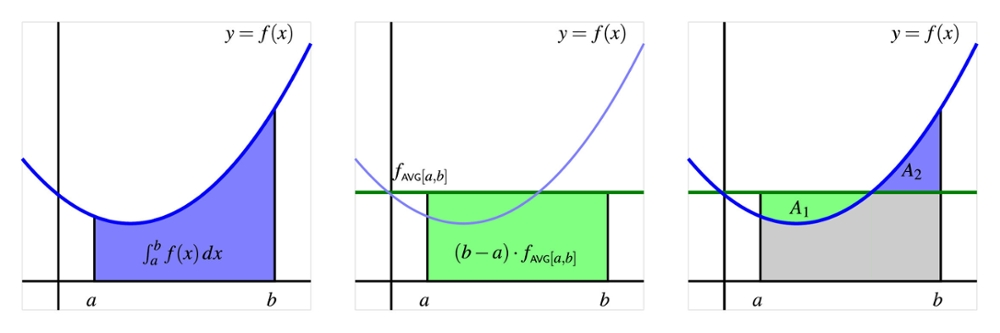
\includegraphics[width=0.7\linewidth]{average-value}
        \caption{Visual inspection of the Average Value Theorem.}
        \label{fig:AVT}
    \end{figure}
    
    So, we can \href{https://www.geeksforgeeks.org/monte-carlo-integration-in-python/}{device an algorithm} that takes values of the function and obtain their average to estimate the value of the requested integral. 

\begin{lstlisting}
from scipy import random 
import numpy as np 
        
a = -np.pi
b = np.pi 
N = 1000
        
ar = np.zeros(N) 
        
for i in range (len(ar)): 
    ar[i] = random.uniform(a,b) 
        
integral = 0.0
        
def f(x): 
    return np.cos(x) 
        
for i in ar: 
    integral += f(i) 
        
ans = (b-a)/float(N)*integral 
        
print ("Approx to the integral by CMC: {}.".format(ans)) 
\end{lstlisting}

\end{frame}

\begin{frame}{Central limit theorem}
    In many situations, for independent and identically distributed (iid) random variables, the sampling distribution of the standardized sample mean tends towards the standard normal distribution even if the original variables themselves are not normally distributed.
    \\[10pt]
    Thus, $\bar{Y}$ approximately has a $\mathcal{N}(\mu,\,\sigma^{2}/N)$ distribution for large $N$, provided that $\mathrm{Var} Y < \infty$.
    \\[10pt]
    Thus we can construct an approximate $(1-\alpha)$ confidence interval for $\mu$:
    \[
        \left(\bar{Y}-z_{1-\alpha/2}\frac{S}{\sqrt{N}}, \bar{Y}+z_{1-\alpha/2}\frac{S}{\sqrt{N}}\right)    
    \]
    where $S$ is the sample standard deviation of ${Y_i}$ and $z_{\gamma}$ is the $\gamma$-quantile of the $\mathcal{N}(0,1)$ distribution. Estimated standard error: $S/\sqrt{N}$; estimated relative error: $S/(\bar{Y}\sqrt{N})$.
\end{frame}

\begin{frame}[fragile]{Algorithm for CMC}
    \begin{algorithm}[H]
        \DontPrintSemicolon
          
        \KwInput{Random variable $Y\sim f$, sample size $N$, confidence level $1-\alpha$.}
        \KwOutput{Point estimate and approximate $(1-\alpha)$ confidence interval for $\mu=\Exp Y$.}
        Simulate $Y_1,\ldots,Y_N \stackrel{iid}{\sim}f$\;
        $\bar{Y}\leftarrow \frac{1}{N}\sum_{i=1}^N Y_i$\;
        $S^2 \leftarrow \frac{1}{N-1}\sum_{i=1}^N (Y_i-\bar{Y})^2$\;
        \Return{$\bar{Y}$ and conf. interval $\left(\bar{Y}-z_{1-\alpha/2}\frac{S}{\sqrt{N}}, \bar{Y}+z_{1-\alpha/2}\frac{S}{\sqrt{N}}\right)$}\;
        \caption{CMC for iid}
        \end{algorithm}
\end{frame}

\begin{frame}{Monte Carlo integration}
    Consider the complicated integral
    \[
        \mu = \int_{-\infty}^{infty}  \int_{-\infty}^{infty} \int_{-\infty}^{infty} \sqrt{|x_1+x_2+x_3|} e^{-(x_1^2+x_2^2+x_3^2)/2} \diff x_1 \diff x_2 \diff x_3  
    \]
    Defining $Y=|X_1+X_2+X_3|^{1/2}(2\pi)^{3/2}$ with $X_1,X_2,X_3 \stackrel{iid}{\sim} \mathcal{N}(0,1)$, we can write $\mu=\Exp Y$.
    Use the code \href{https://biocomputing-teaching.github.io/Data-Science-with-Python/code/UNIT3-MC-Methods.html}{here} to test the calculation. If you want to learn more about CLT and confidence intervals, a good start can be found \href{https://online.stat.psu.edu/stat506/lesson/1/1.4}{here}.
\end{frame}

\begin{frame}{Polynomial regression. Original data.}
  \begin{figure}
    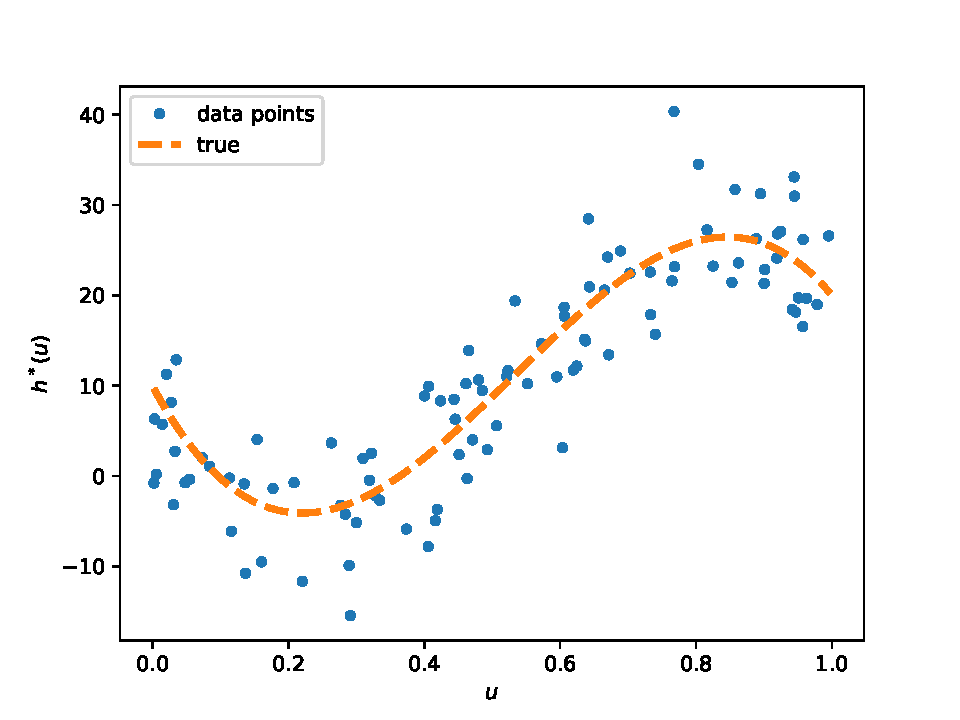
\includegraphics[width=0.7\linewidth]{polydatpy}
    \label{fig:polydatpy}
    \caption{Training data and the optimal polynomial prediction function $h^*$\cite{kroese2020}.}
  \end{figure}
\end{frame}

\begin{frame}{Polynomial regression. Estimating the generalization risk}
    The code \href{https://biocomputing-teaching.github.io/Data-Science-with-Python/code/UNIT3-MC-Methods.html}{here} shows how to estimate how good is the graph below. 
  \begin{figure}
    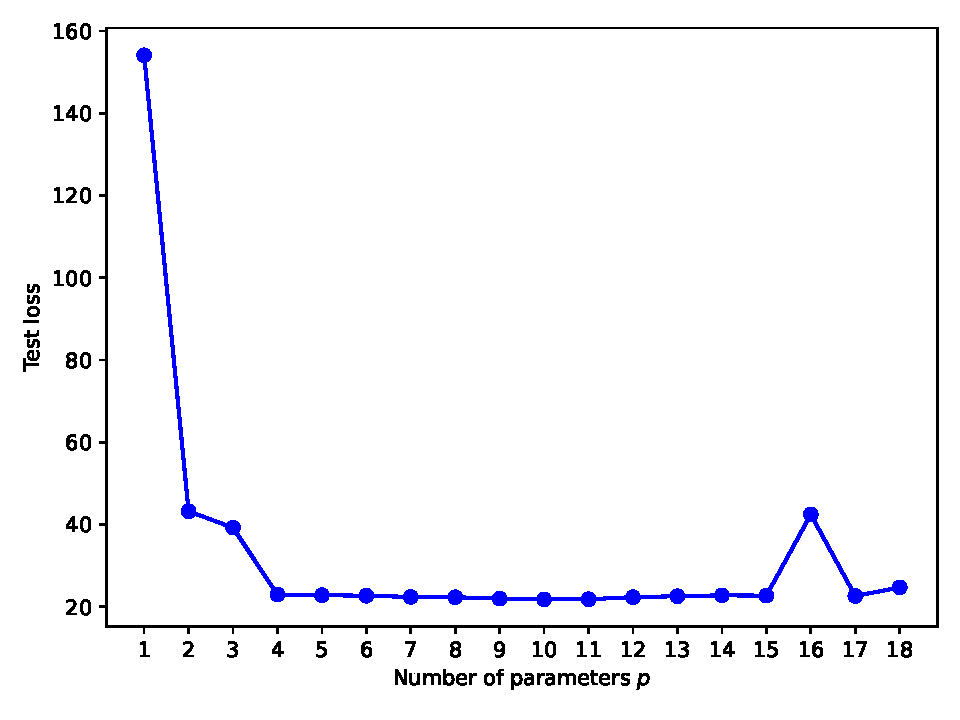
\includegraphics[width=0.4\linewidth]{MSEpy}
    \label{fig:crossvalpy}
    \caption{Fitted models for different orders of polynomial regressions\cite{kroese2020}.}
  \end{figure}
\end{frame}

\section{Bibliography}
\bibliographystyle{unsrt}
\bibliography{DataSciencewithPython}
\end{document}